\chapter{Design \& Methodology}

This chapter will discuss/detail/etc ...
%todo

\section{Methodology}
A Scrum-like software development methodology was used for the duration of this project, along with elements from the Kanban method.

Scrum is a kind of Agile development methodology that is based on a series of iterative cycles of development called \emph{sprints}. These sprints will often begin with a brief planning session, can last from 1 to 4 weeks, then finish with a sprint retrospective to review how it went.

% todo: ref scrum
% todo: Fix tenses in this section

Scrum is usually a heavily team-based process, involving several roles such as `Scrum Master`, `Product Owner' and the Scrum team. Daily 15 minute team meetings are held to assess how the sprint is going, with each role and team member talking about what they did and what they plan to do. Since this project will be completed by a single person, I will be focusing on the iterative development, planning and review aspects of the Scrum methodology rather than the daily meetings and roles.

% todo: http://www.mountaingoatsoftware.com/agile/scrum

Using an Agile methodology like Scrum means that most of the design of the application will be done as needed, rather than up front such as in the waterfall model. Design documents such as  entity-relationship diagrams will be completed as they become necessary for the continuation of the development process, or if another part of the project depends on the design being completed.

\subsection{Project Management}
A \emph{kanban board} will be used to manage tasks during each sprint. Trello will be used as the board by adding a list for each iteration in the development process. Cards will be added to these lists for each task, and labels will be used as kanban columns by using labels such as `Ready', `In Progress', and `Completed' as can be seen in Figure \ref{fig:kanban}. If cards are overdue, they can be moved to the next sprint list as a backlog, by dragging and dropping.

% todo: Ref kanban

\begin{figure}[h]
	\centering
	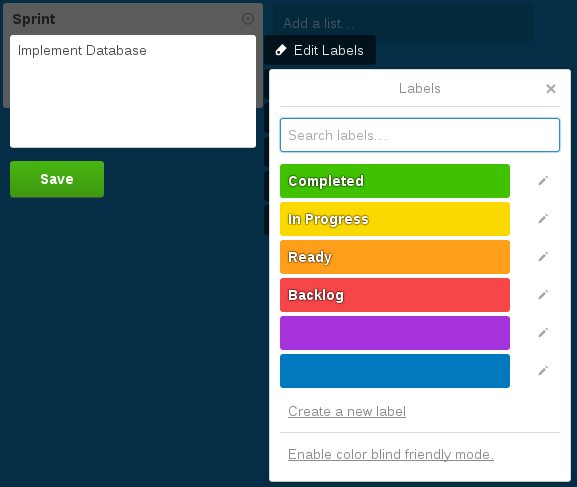
\includegraphics[scale=0.7]{kanban}
	\caption{Kanban-style task labels in Trello}
	\label{fig:kanban}
\end{figure}

%todo: fix branching

Git will be used throughout the development process to provide version control and project management through branches. Branching will be used to manage the status of the project via stable and development branches. The Git repository will be hosted both locally and remotely on GitHub for a backup.

\section{User Interface}
% Usability, how being on the web affected interface design
	\subsection{Main website} % todo

	% todo wording
	The website will be what the user interacts with initially when they visit the web application, where they are able to browse games published by other users or manage their own games. Neilsen's heuristics were taken into consideration while designing this portion of the application, leaning strongly towards aesthetic and minimal design while creating the user interface.  
	% todo {website}
	% todo ref Neilsen's Heuristics

	\paragraph{Horizontal Prototype.}
	In order to begin developing the website for this project, a medium fidelity horizontal prototype was created. The horizontal prototype allowed me to examine how the user would interact with the system, and visualise the actions that the user will perform while using it.

	% todo ref

	% todo figures
	\begin{figure}[h]
		\centering
		
\includegraphics[scale=0.3]{placeholder}
		\caption{Front page horizontal prototype}
		\label{fig:frontpageprototype}
	\end{figure}

	\begin{figure}[h]
		\centering
		
\includegraphics[scale=0.3]{placeholder}
		\caption{Dashboard horizontal prototype}
		\label{fig:dashboardprototype}
	\end{figure}

	Figure \ref{fig:frontpageprototype} shows the horizontal prototype design for the front page of the website. This shows the actions available to a guest on the system; such as logging in, or browsing the games published by other users on the system. The user is able to click `Play' on one of the available games to launch into a new page where they can play that game.

	Figure \ref{fig:dashboardprototype} shows the design of the dashboard; where logged in users can manage their games on the system. The dashboard allows logged in users to add a new game project, delete an existing one, launch into the editor for a project, or playtest their game. There are also actions available to clone a repository from GitHub, make commits, and push \& pull an existing project to and from GitHub.

	\subsection{Game Editor}
	The game editor will be the most important part of the website, where users will be able to construct scenes for their games by creating new scenes, entities and components. The interface for this part of the web application was designed to be similar in regards to the Unity game editor; as it provides a familiar experience for those who have used it. It was also designed with Neilsen's heuristics in mind, aiming for a high usability rating.

	\paragraph{Horizontal Prototype.}
	The prototype for the game editor can be seen in Figure \ref{fig:gameeditorprototype}. The layout of the editor is split into three columns; the \emph{explorer}, \emph{scene}, and \emph{properties}. There are also tabs that will contain a script editor, allowing the user to switch to it and create their own custom components.

	% todo fig
	\begin{figure}[h]
		\centering
		
\includegraphics[scale=0.3]{placeholder}
		\caption{Dashboard horizontal prototype}
		\label{fig:gameeditorprototype}
	\end{figure}

	\paragraph{Explorer.}
	In the explorer, a tree of the current game is displayed, where scenes contain a list of entities, and entities contain a list of components. Actions can be performed on these scenes, entities and components such as adding, deleting or copying.

	\paragraph{Scene.}
	The scene is the centerpiece of the editor, which displays a visualisation of the currently selected scene along with all entities inside of it. The scene view updates realtime with any changes that are made in the editor, providing feedback to the user when they add, delete or change properties on an entity.

	\paragraph{Properties.}
	The properties list shows a list of the components and their respective properties for the selected entity in the explorer. Here the user will be able to change the properties of components on entities; such as colours, position, scale, and rotation. When property changes are made, the scene will update accordingly.

	\subsection{Final designs}
	% Pictures
	% How they changed slightly, using bootstrap, etc

\section{System Components}
	\subsection{Overview}
	% Overview of entire system
	% Overview of network

% MongoDB?

	\subsection{Storage Server}
	% Rest API, planned routes
	% Folder structure for storing files /user/repo

	\subsection{Web Server}
	% Structure

	\subsection{Game Engine}
	% Scene, Entity, Component relationship
	% Default components ^

	\subsection{Game Editor}

\section{Use Cases \& Features}
% Clearly identify the list of features and use cases supported within the project